\numericsubsection{Downwind Scheme}

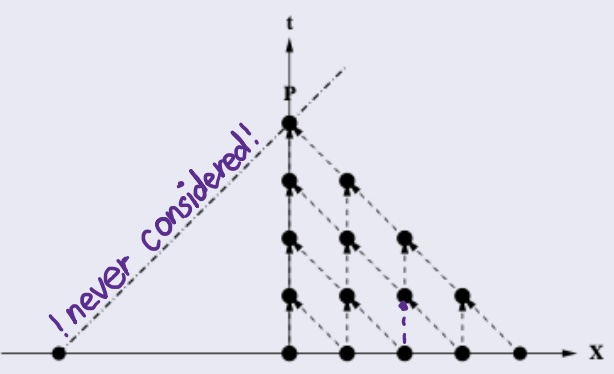
\includegraphics[width=0.3\columnwidth]{images/downwind_scheme}

{\color{orange}\faWarning\ This scheme will in general diverge and frankly is \faTrash.}

\begin{enumerate}
	\item \emph{Discretisation of operators} of PDE $Lu(...)=f(...)$
	\item{
		\emph{Discretise geometry} by introducing a grid:
		$x_{j,k} = (j\cdot\Delta x, k\cdot\Delta t)$ with $j$ as the local index
		and $k$ as the time index where $k=0$ is on boundary
		and \colorbox{shadecolor}{$\Delta x = \frac{1}{n}$},
		\colorbox{shadecolor}{$\Delta t = \frac{r}{n}$}
		and \colorbox{shadecolor}{$r = \frac{\Delta t}{\Delta x}$} 
		({\color{orange}\faWarning} in contrast to $r=\Delta t\div\Delta x^2$ for parabolic equations)
	}
	\item{
		\emph{Find matrix $\utild_{j,k}$} satisfying discretised equation for inner grid points
		and $\utild_{j,0}=f_j$ on boundary
	}
\end{enumerate}

\subsubsection{Example Using Advection Equation}

\textbf{Given} the advection equation 
$\frac{\partial u}{\partial x} + \frac{\partial u}{\partial t} = 0$ on
$\Omega = (-\infty,\infty)\times[0,\infty)$ with Dirichlet's boundary condition
$u(x,0) = f(x) = e^x$. We want to get approximation $\utild(0,1)$ using
$\Delta x = \sfrac{1}{4}$ and $\Delta t = \sfrac{1}{4}$.
\\[1em]
\textbf{Discretisation of Operators}
\begin{align*}
	& \left.{\frac{\utild(x,t+\Delta t)-\utild(x,t)}{\Delta t}}
	+ {\frac{\utild(x+\Delta x,t)-\utild(x,t)}{\Delta x}} = 0\quad\right|\cdot \Delta t \\
	& (\utild(x_{j,k+1})-\utild(x_{j,k}))+r(\utild(x_{j+1,k})-\utild(x_{j,k}))=0
	{\color{gray} \quad(\Delta t\div\Delta x = r)}
\end{align*}
\colorbox{shadecolor}{$
	\displaystyle
	\Rightarrow \utild_{j,k+1}
	= \left(1+r\right)\cdot\utild_{j,k}-r\cdot\utild_{j+1,k}
	{\color{gray}\quad\text{(= discrete advection eq.)}}
$}

\textbf{Discretisation of Geometry}

\makebox[\columnwidth]{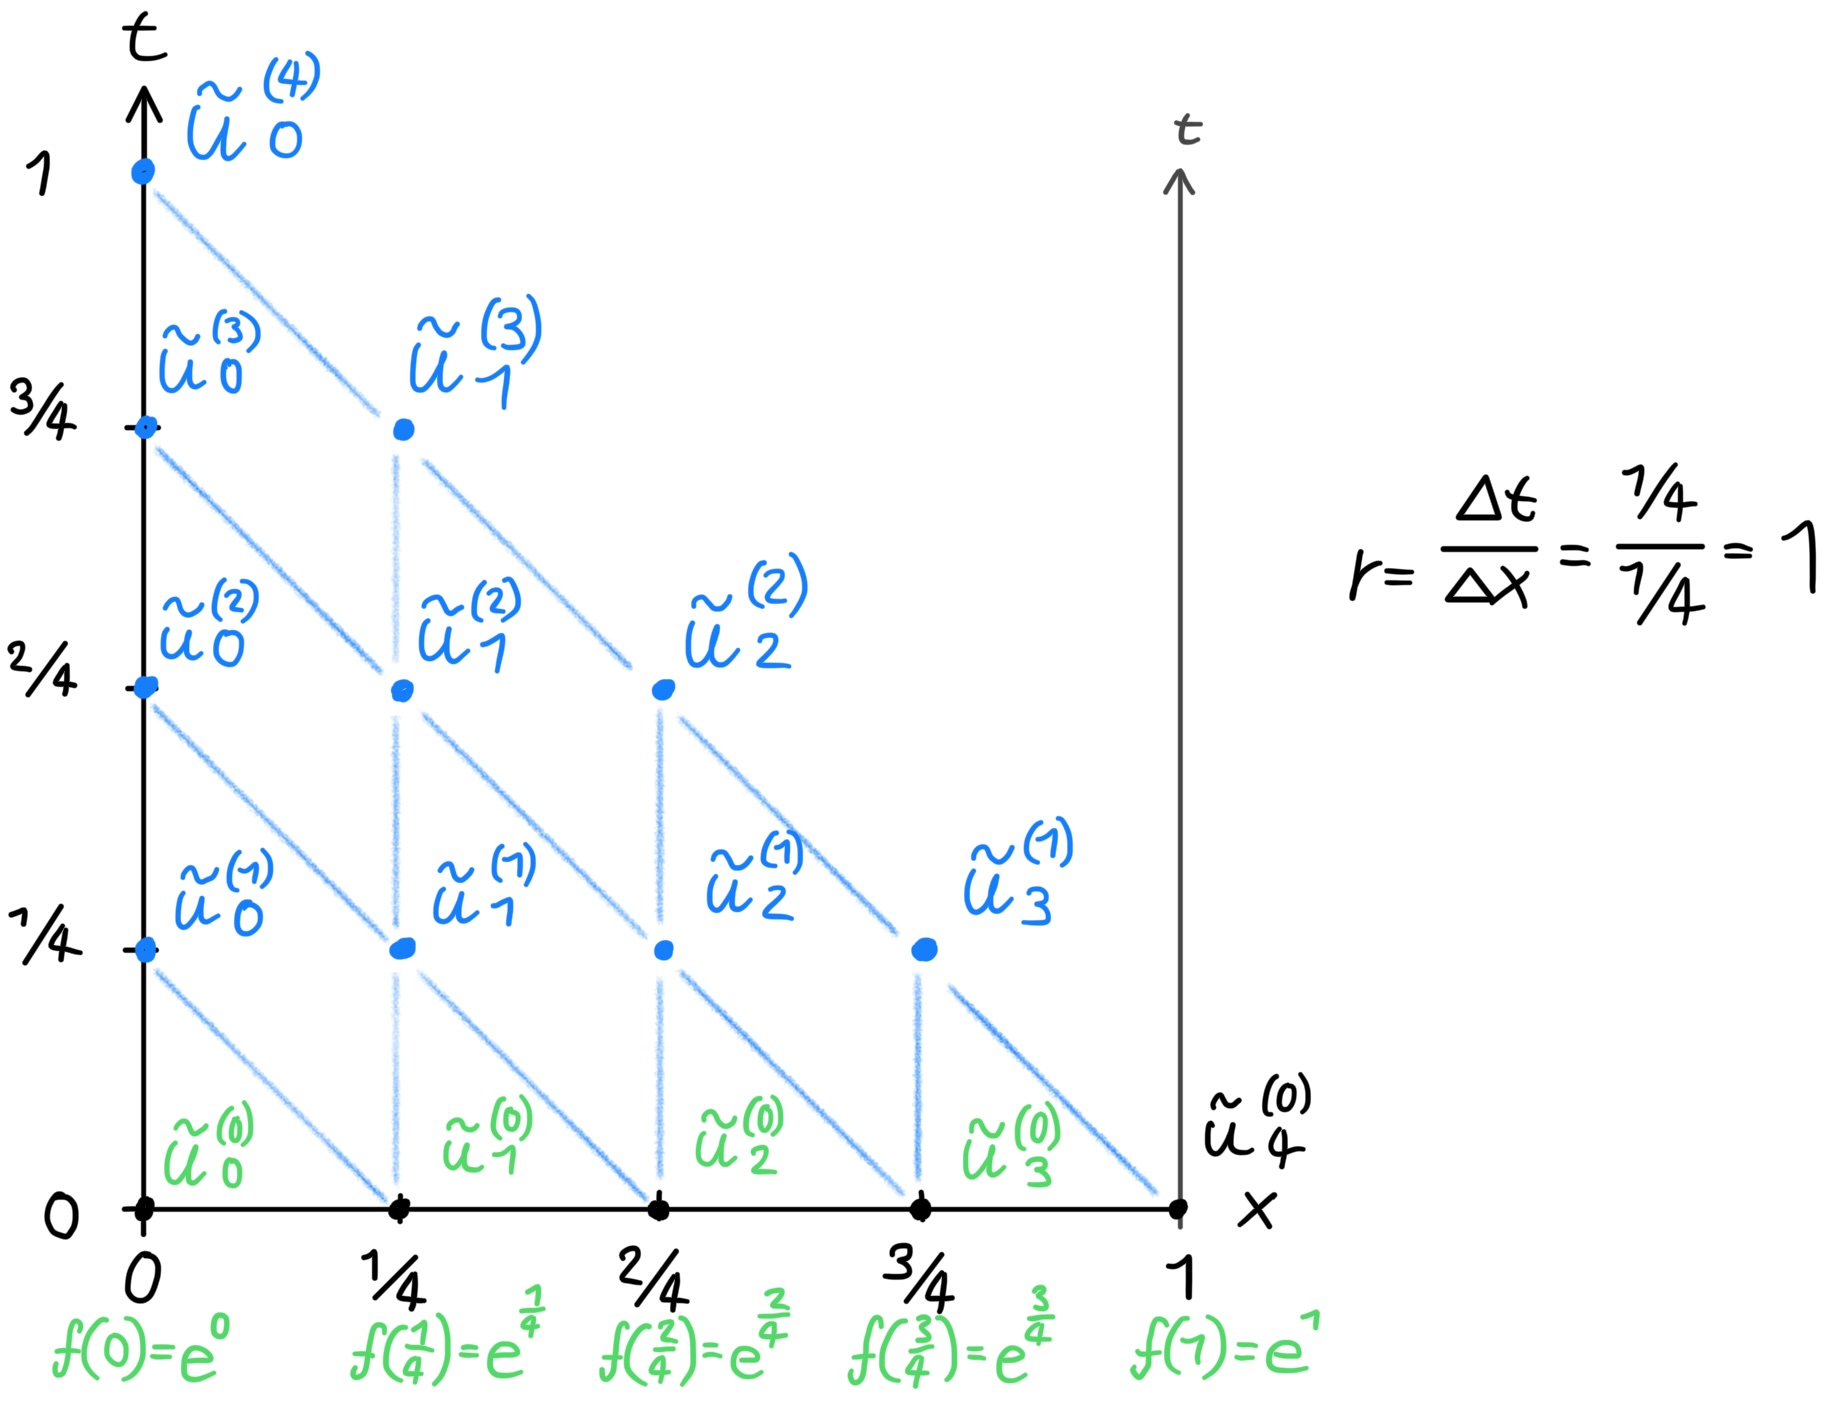
\includegraphics[width=0.6\columnwidth]{images/downwind_scheme_geometry}}

\textbf{Solution} Apply discrete advection eq. until $u_0^{(4)}$ is reached.